% !TEX encoding = UTF-8 Unicode
\documentclass[
10pt,
aspectratio=169,
]{beamer}
\setbeamercovered{transparent=10}
\usetheme[
%  showheader,
%  red,
  purple,
%  gray,
%  graytitle,
  colorblocks,
%  noframetitlerule,
]{Verona}

\usepackage[T1]{fontenc}
\usepackage[utf8]{inputenc}
\usepackage{lipsum}
%%%%%%%%%%%%%%%%%%%%%%%%%%%%%%%
% Mac上使用如下命令声明隶书字体,windows也有相关方式,大家可自行修改
%\providecommand{\lishu}{\CJKfamily{zhli}}
%%%%%%%%%%%%%%%%%%%%%%%%%%%%%%%
\usepackage{tikz}
\usetikzlibrary{fadings}
%
%\setbeamertemplate{sections/subsections in toc}[ball]
%\usepackage{xeCJK}
\usepackage{adjustbox} % Shrink stuff
\usepackage{listings}
\usepackage{caption}
\usepackage{subcaption}
\usefonttheme{professionalfonts}
\def\mathfamilydefault{\rmdefault}
\usepackage{amsmath}
\usepackage{multirow}
\usepackage{booktabs}
\usepackage{bm}
\setbeamertemplate{section in toc}{\hspace*{1em}\inserttocsectionnumber.~\inserttocsection\par}
\setbeamertemplate{subsection in toc}{\hspace*{2em}\inserttocsectionnumber.\inserttocsubsectionnumber.~\inserttocsubsection\par}
\setbeamerfont{subsection in toc}{size=\small}
\AtBeginSection[]{%
	\begin{frame}%
		\frametitle{Outline}%
		\textbf{\tableofcontents[currentsection]} %
	\end{frame}%
}

\AtBeginSubsection[]{%
	\begin{frame}%
		\frametitle{Outline}%
		\textbf{\tableofcontents[currentsection, currentsubsection]} %
	\end{frame}%
}

\title{B\'usqueda y revisi\'on bibliografica}
\subtitle{Herramientas para la elaboraci\'on de la propuesta}
\author[L.M.]{Luis Alejandro Morales, Ph.D.}
\mail{lmoralesm@unal.edu.co}
\institute[UNAL]{Facultad de Ingenier\'ia, Departamento de Ingnenier\'ia Civil y Agr\'icola\\
Universidad Nacional de Colombia, Bogot\'a}
\date{\today}
\titlegraphic[width=3cm]{logo_01u}{}

%%%%%%%%%%%%%%%%%%%%%%%%%%%%%%%%
% ----------- 标题页 ------------
%%%%%%%%%%%%%%%%%%%%%%%%%%%%%%%%
% New commands
\newcommand{\gi}{\texttt{Git}}
\newcommand{\gih}{\texttt{GitHub}}
\newcommand{\co}[1]{\alert{\textbf{\large \texttt{#1}}}}
\begin{document}



\maketitle

%%% define code
\defverbatim[colored]\lstI{
	\begin{lstlisting}[language=C++,basicstyle=\ttfamily,keywordstyle=\color{red}]
	int main() {
	// Define variables at the beginning
	// of the block, as in C:
	CStash intStash, stringStash;
	int i;
	char* cp;
	ifstream in;
	string line;
	[...]
	\end{lstlisting}
}
%%%%%%%%%%%%%%%%%%%%%%%%%%%%%%%%
% ----------- FRAME ------------
%%%%%%%%%%%%%%%%%%%%%%%%%%%%%%%%

%---
\section{Manejadores de referencias}

\begin{frame}[c]{Importancia de los manejadores de referencia}
\begin{itemize}
\item Incrementa la productividad.
\item Organiza la bibliograf\'ia y disminuye la posibilidad de plagio.
\item Mejora la calidad de las citas en el texto.
\item Permite la toma de notas sobre documentos consultados.
\item Almacena PDFs de art\'iculos. Hace la b\'usqueda de estos. 
\item Intuitivos y f\'aciles de usar.
\end{itemize}
\end{frame}


\begin{frame}[c]{Manejadores de referencia}
Existen diferentes manejadores de referencia. Los m\'as comunes son:
\begin{table}
\begin{adjustbox}{width=\textwidth}
\begin{tabular}{ l c c c }
& \textbf{Disponibilidad} & \textbf{Compatibilidad} & \textbf{Otros}\\
 \href{https://www.zotero.org/}{\alert{Zotero}} & Free. Web-based \& desktop & MS Word, OpenOffice \& Google docs & Popular\\
 \href{https://www.mendeley.com/}{\alert{Mendeley}} & Free. Web-based \& desktop & MS Word \& OpenOffice & Popular \\
 \href{https://endnote.com/es/}{EndNote} & Lisenced. Web-based \& desktop (independent) & MS Word & M\'as sofisticado \\
 \href{https://refworks.proquest.com/}{RefWorks}: & Lisenced. Web-based & MS Word \& Google docs & Large databases \\
 \href{https://www.citavi.com/en}{Citavi} & Lisenced. Web-based \& desktop (independent) & MS Word \& Google docs & Popular in Germany 
\end{tabular}
\end{adjustbox}
\end{table}
\end{frame}

%---
\section{Lectura eficiente}
\begin{frame}[c]{Lectura activa y eficiente}
La lectura activa:
\begin{columns}
\column{0.3\textwidth}
\begin{itemize}
\item Es selectiva
\item Es cr\'itica
\item Interact\'ua con el texto
\item Cambia el orden de lectura
\item Se lee con un prop\'osito
\item Anticipa
\end{itemize}
\column{0.8\textwidth}
\centering
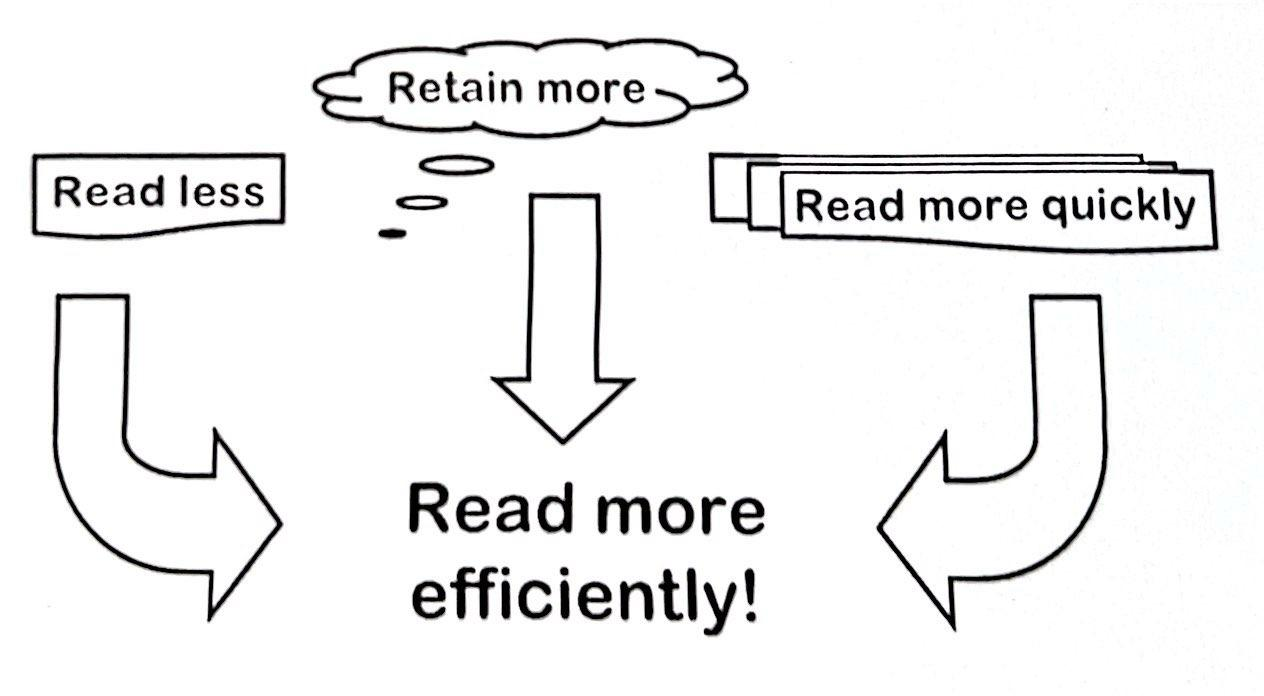
\includegraphics[width=\textwidth]{fig1.jpeg}
\end{columns}
\end{frame}

\begin{frame}[c]{Pasos}
\centering
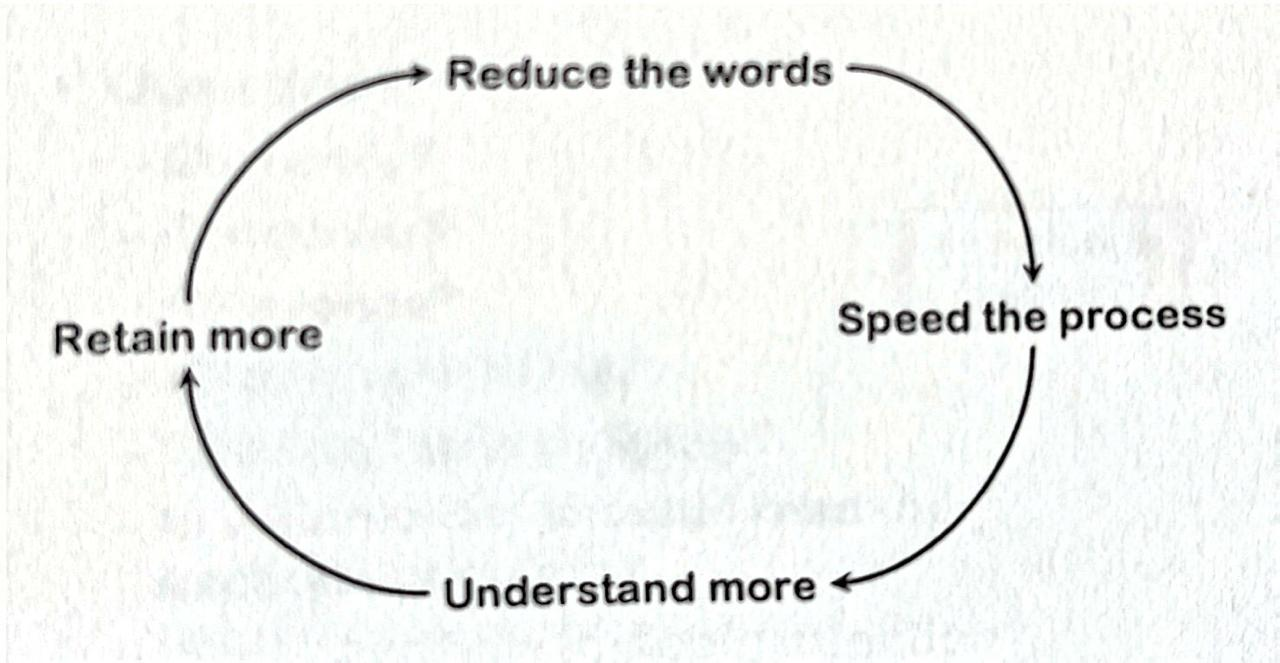
\includegraphics[width=\textwidth]{fig2.jpeg}
\end{frame}

\begin{frame}[c]{Seleci\'on}
Preguntas a formularse antes y durante la lectura
\begin{itemize}
\item ¿Aceptaci\'on, diseminaci\'on?
\item ¿Credibilidad?
\item ¿Relevancia?
\item ¿Que es nuevo para mi?
\item ¿Que conozco ya?
\item ¿En que orden debo leer las secciones/cap\'itulos?
\item ¿Que necesita mayor atenci\'on?
\end{itemize}
\end{frame}


\begin{frame}[c]{Organizaci\'on}
Tomar notas y organizarlas de acuerdo con:
\begin{itemize}
\item Palabras claves
\item Parafrasear ideas
\item Comparaci\'on con otros trabajos
\item Opinar con criterio
\item Formular preguntas sobre el texto
\item Map\'eo de la informaci\'on
\end{itemize}
\end{frame}

\begin{frame}[c]{Aceleraci\'on}
Problemas en la velocidad de lectura:
\begin{itemize}
\item Subvocalizaci\'on
\item Vuelta atr\'as
\item Interrupciones
\item Luz baja e incomodidad
\item Fatiga y cansancio
\item Vocabulario pobre y mala comprensi\'on
\item Sesiones largas de lectura
\end{itemize}
Curas simples:
\begin{itemize}
\item Mejorar la postura y comodidad
\item Buena luz
\end{itemize}
\end{frame}


\begin{frame}[c]{¿Porque la copia impresa es mejor?}
\begin{itemize}
\item Las anotaciones son flexibles y f\'aciles
\item Navegar el documento es mas f\'acil
\item Es m\'as recomendable cuando se hacen m\'ultiples tareas
\item F\'acil para manejar/consultar varios documentos
\end{itemize}
\end{frame}

\begin{frame}[c]{Retenci\'on}
\alert{SMART} reading:
\alert{S}pecific \alert{M}apped \alert{A}chievable  \alert{R}elevant \alert{T}ime-limited 
Pasos en el proceso de lectura:
\begin{enumerate}
\item Map\'eo y revisi\'on
\item Vista anticipada
\item Escaneo, ojeado: Anticipar la estructura y el contenido.
\item Lectura y notas: Preparar tu sitio de trabajo, alcance de la lectura, materiales, etc.
\item Revisi\'on y reflexi\'on
\end{enumerate}
\end{frame}


\begin{frame}[c]{Concentraci\'on y comprensi\'on}
\begin{table}
\begin{adjustbox}{width=\textwidth}
\begin{tabular}{ c c }
\textbf{Concetraci\'on} & \textbf{Comprensi\'on}\\
Determinar objetivos espec\'ificos & Mejorar tu vocabulario (prefijos, sufijos, t\'erminos t\'ecnicos) \\
Programacion real lectura & Remover distracciones \\
Leer puntual & Reducir fijaciones por linea \\
Leer en el mismo sitio & 
\end{tabular}
\end{adjustbox}
\end{table}
¿Que se retiene?
\begin{itemize}
\item Conceptos significativos e importantes
\item Conceptos familiares o \'unicos
\item Conceptos f\'aciles de mapear
\end{itemize}
\end{frame}


\begin{frame}[c]{¿Como trabaja la memoria y el cerebro?}
La memoria se mejora:
\begin{columns}
\column{0.4\textwidth}
\begin{itemize}
\item Atenci\'on e inter\'es
\item Organizaci\'on 
\item Practica
\end{itemize}
\column{0.6\textwidth}
\centering
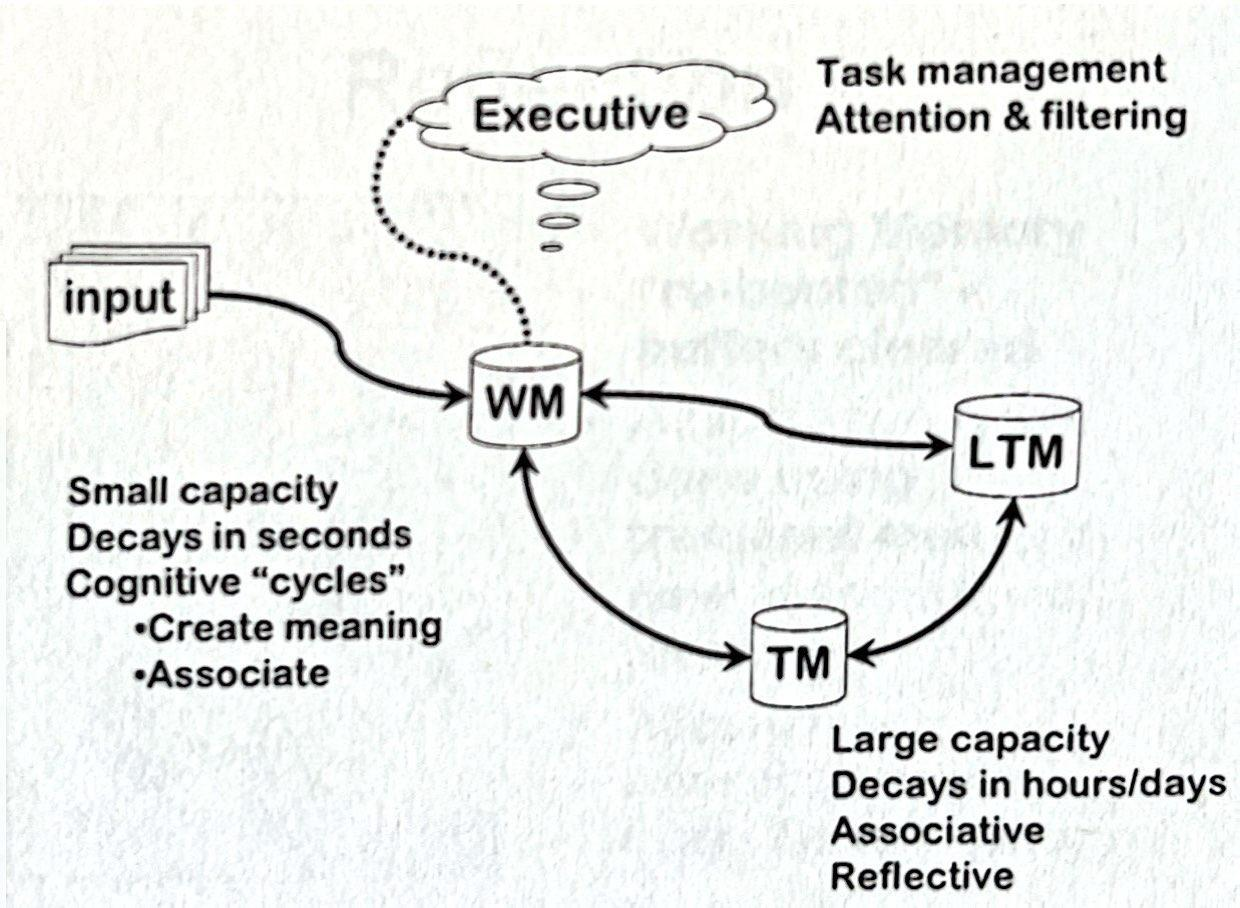
\includegraphics[width=\textwidth]{fig3.jpeg}
\end{columns}
\end{frame}


\begin{frame}[c]{Retenci\'on}
Como mejorarla:
\begin{itemize}
\item Restablecer y limpiar la \alert{memoria de trabajo}
\item Asociar la lectura usando la \alert{memoria transitoria} y las nuevas asociaciones creadas
\item Permitir interacciones mas libres con la \alert{memoria de largo plazo}
\end{itemize}
\end{frame}

%---
\section{Revisi\'on de la literatura}
\begin{frame}[c]{¿Que es la revisi\'on de la bibliograf\'ia?}
\begin{block}{Definici\'on}
Es el proceso de explorar la literatura para establecer el \alert{status quo} y formular una hip\'otesis o pregunta de investigaci\'on, la cual se justifica a trav\'es de la comparaci\'on con otros trabajos. La revisi\'on deber ser una s\'intesis del trabajo de otros.
\end{block}
\begin{itemize}
\item Una evaluación organizada y crítica de publicaciones para responder una pregunta
\item No es simplemente un catalogo descriptivo de publicaciones
\item Por lo tanto, es importante conocer y entender la pregunta de investigaci\'on
\end{itemize}
\end{frame}

\begin{frame}[c]{Preguntas claves sobre la revisi\'on}
\begin{itemize}
\item ¿Que es lo que sabemos?
\item ¿Que es lo que N\'O sabemos?
\item ¿Que ha sido intentado/probado?
\item ¿Funciona?
\item ¿Que ha sido discutido?
\item ¿Que no se ha hecho?
\item ¿Que es lo que yo intento hacer?
\item ¿Que tan importante es?
\end{itemize}
\end{frame}


\begin{frame}[c]{¿Cual es el prop\'osito de la revisi\'on?}
\begin{itemize}
\item Dar una mirada a los grandes problemas o temas de trascendentales
\item Seleccionar alguno de estos como estudio
\item Resumir el trabajo de otros
\item Evaluar el trabajo de otros
\item Proporcionar contexto a la idea de investigaci\'on
\item Indentificar vac\'ios
\item Entender teor\'ias y m\'etodos
\end{itemize}
\end{frame}


\begin{frame}[c]{Fundamentos de la revisi\'on bibliogr\'afica}
\begin{itemize}
\item La pregunta de investigaci\'on
\item Alcance de la revisi\'on
\item Organizaci\'on de la revisi\'on:
\begin{itemize}
\item Cronol\'ogica
\item Tem\'atica (E.j. modelos, resultados, regiones, etc)
\item Metodol\'ogica
\end{itemize}
\end{itemize}
\end{frame}


\begin{frame}[c]{¿Como se juzga la revisi\'on bibliogr\'afica?}
\begin{itemize}
\item ¿Encontr\'o toda la literatura relevante?
\item ¿La revisi\'on ha sido ordenada apropiadamente?
\item ¿Entendi\'o todo lo que ley\'o?
\item ¿Escribi\'o una opini\'on critic\'o lo que ley\'o?
\item ¿Identific\'o, defini\'o y justific\'o la investigaci\'on que desea realizar?
\end{itemize}
\end{frame}

\begin{frame}[c]{Fases de la revisi\'on bibliogr\'afica}
\centering
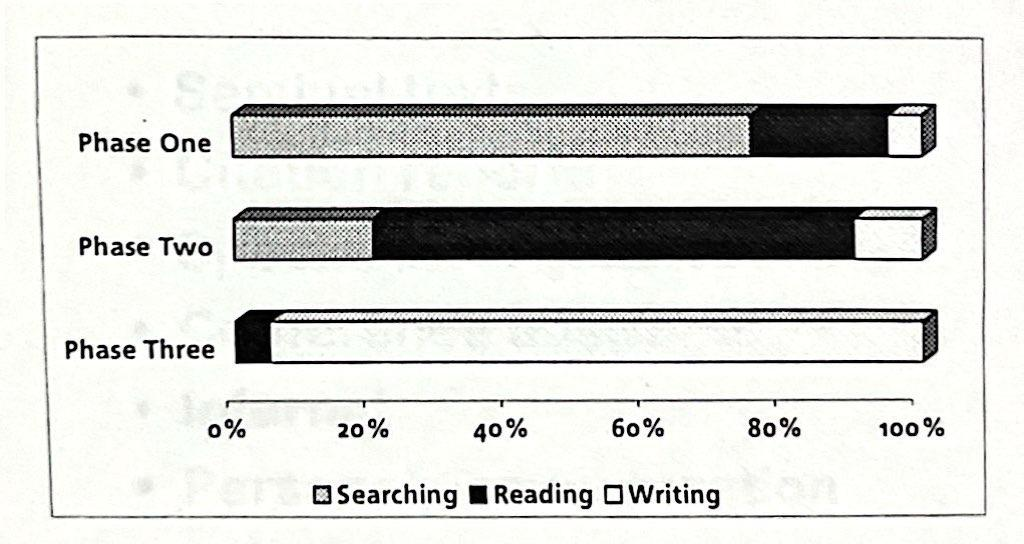
\includegraphics[width=\textwidth]{fig4.jpeg}
\end{frame}


\begin{frame}[c]{¿Como se siente haciendo la revisi\'on bibliogr\'afica?}
\begin{table}
%\begin{adjustbox}{width=\textwidth}
\begin{tabular}{ c p{.5\linewidth} p{.4\linewidth} }
$-$ & Ignorante, confundido, abrumado & $\longrightarrow$ Aprender que es lo esta all\'i \\
& Capaz de entender el problema y algunas de las soluciones & $\longrightarrow$ Inicio de la selecci\'on \\
& Capaz de hacer juicios sobre lo que ha le\'ido & $\longrightarrow$ Lectura activa; toma de notas \\
$+$ & Seguro de realizar una organizada y critica revisi\'on de la literatura & $\longrightarrow$ Visualizaci\'on de la organizaci\'on de la revisi\'on 
\end{tabular}
%\end{adjustbox}
\end{table}
\end{frame}

\begin{frame}[c]{La busqueda}
Iniciando la busqueda:
\begin{itemize}
\item Libros de texto
\item Reportes de citaciones
\item Revistas especializadas
\item Res\'umenes de conferencias
\item Internet
\item Comunicaciones personales 
\end{itemize}
¿Que es relevante?
\begin{enumerate}
\item El t\'itulo
\item El abstract y palabras claves
\item La fecha de publicaci\'on
\item Las citaciones
\item La revista
\end{enumerate}
\end{frame}


\begin{frame}[c]{¿Como leer un art\'iculo?}
\begin{enumerate}
\item Leer el t\'itulo
\item Leer el abstract y las palabras claves
\item Leer las conclusiones
\item Decidir que partes leer a profundidad
\begin{itemize}
\item ¿Leer la introducci\'on?
\item ¿Leer los resultados?
\item ¿Leer la metodolog\'ia?
\item ¿Leer la discusi\'on?
\end{itemize}
\end{enumerate}
\end{frame}

\begin{frame}[c]{¿Que preguntas hacerse al leer un articulo?}
\begin{itemize}
\item ¿Cual es el objetivo, pregunta de investigaci\'on o hipot\'esis?
\item ¿Cuales son lo resultados de la investigaci\'on?
\item ¿Que metodolog\'ias, estrategias o teor\'ias son empleadas?
\item ¿En que contexto se realiz\'o la investigaci\'on?
\item ¿Cual es la contribuci\'on al \'area de estudio?
\item ¿Como se relaciona con mi pregunta de investigaci\'on?
\end{itemize}
\end{frame}
%---

\section{Escritura de la revisi\'on bibliogr\'afica}
\begin{frame}[c]{Organizaci\'on}
\begin{enumerate}
\item Decidir como organizar la revisi\'on:
\begin{itemize}
\item ¿Cronol\'ogica?
\item ¿Tem\'atica?
\item ¿Metodol\'ogica?
\end{itemize}
\item Escribir la estructura de la revisi\'on
\end{enumerate}
\end{frame}


\begin{frame}[c]{Estructura de la revisi\'on}
\begin{itemize}
\item Introducci\'on
\begin{itemize}
\item Tener en mente la pregunta de investigaci\'on
\item Resumen de intentos previos por resolverla
\end{itemize}
\item Cuerpo de la revisi\'on 
\begin{itemize}
\item Secciones de acuerdo con el m\'etodo de organizaci\'on
\end{itemize}
\item Conclusiones
\begin{itemize}
\item ¿Cuales son los vac\'ios?
\item ¿Vale la pena intentar llenarlos?
\item ¿Quien ha hecho el mayor intento por llenarlos?
\item ¿Como intento llenarlos?
\end{itemize}
\end{itemize}
\end{frame}


\begin{frame}[c]{T\'ecnicas de escritura}
\begin{itemize}
\item Siga la estructura
\item Escriba un primer borrador sin tener muy en cuenta las formas
\item Enf\'oquese en el prop\'osito
\item Recuerde que se requiere
\item Refine su borrador inicial:
\begin{itemize}
\item Espere un par de d\'ias
\item Revise datos importantes
\item Revise redacci\'on, ortograf\'ia y estilo
\item Re-escriba las veces necesaria
\item ¿Suficientes referencias?
\end{itemize}
\item Revise su versi\'on final en copia impresa
\end{itemize}
\end{frame}

%






%\section{?`Que es \gi?}
%\begin{frame}[c]{?`Que es \gi?}
%\begin{columns}
%\column{0.6\textwidth}
%\large{
%\begin{block}{\gi}
%\begin{itemize}
%    \item \gi\ es un programa/sistema usado para el control de versiones en proyectos, particularmente, en c\'odigos de computador.
%    \item \gi\ fue inventado en 2005 por Linus Torvalds, creador de \texttt{Linux}, con el fin de manejar proyectos grandes multiusuario (e.g. kernel de \texttt{Linux} escrito en \texttt{C}) de manera eficiente y r\'apida.
%    \item Git est\'a escrito en \texttt{C} y viene por defecto en \texttt{Linux}. Puede ser instalado en \texttt{MS Windows}.
%\end{itemize}
%\end{block}
%}
%\column{0.4\textwidth}
%\begin{center}
% %\begin{figure}
% 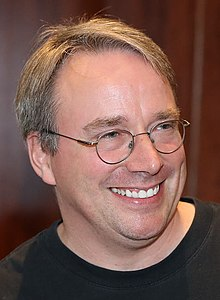
\includegraphics[width=\textwidth]{linus.jpeg}
% %\vspace{-0.5cm}
% %\caption{\tiny Fuente: https://en.wikipedia.org/wiki}
% %\end{figure}
% \end{center}
%\end{columns}
%\end{frame}	
%%---
%\section{?`Para que sirve \gi?}
%\begin{frame}[c]{?`Para que sirve \gi?}
%%\begin{columns}
%%\column{0.6\textwidth}
%\large{
%\begin{block}{Utilidades de \gi}
%\begin{itemize}
%    \item Trabajo en grandes proyectos con colaboracion de multiples usuarios y servidores.
%    \item Control de cambios lo que permite ir a hacia adelante o hacia atras en la historia del proyecto.
%    \item Sistema distribuido lo que permite que multiples usuarios hagan cambios y sean a la vez servidores del proyecto.
%\end{itemize}
%\end{block}
%}
%\end{frame}	
%
%\begin{frame}[c]{Modelo centralizado Vs \alert{modelo distribuido}}
%\vspace{-0.2cm}
%\begin{center}
% 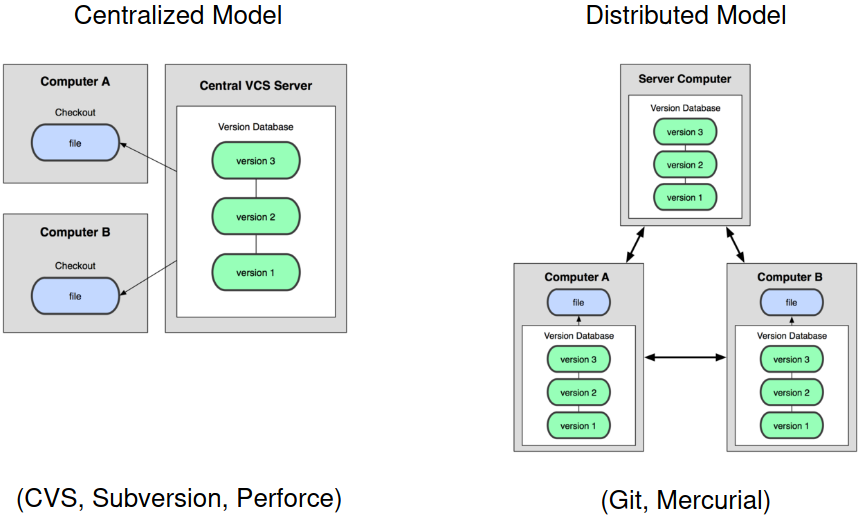
\includegraphics[width=0.87\textwidth]{dist.png}
% \end{center}
%\end{frame}	
%%---
%\section{Tratamiento de cambios en un repositorio en \gi}
%\begin{frame}[c]{Proyecto local en \gi}
%\vspace{-0.2cm}
%\begin{center}
% %\begin{figure}
% 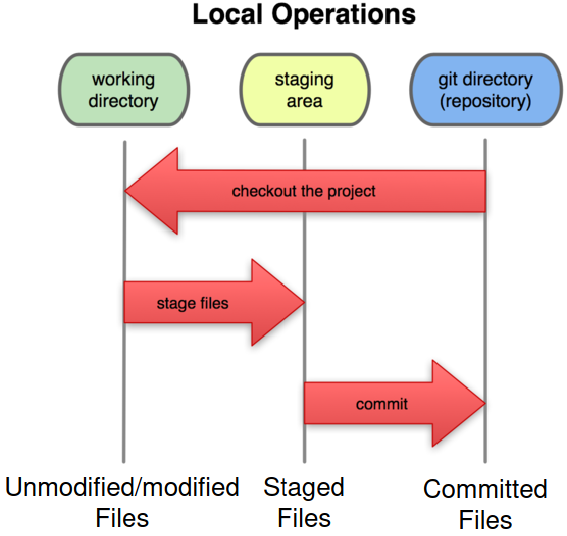
\includegraphics[width=0.55\textwidth]{gitp.png}
% %\vspace{-0.5cm}
% %\caption{\tiny Fuente: https://en.wikipedia.org/wiki}
% %\end{figure}
% \end{center}
%%\end{columns}
%\end{frame}	
%
%\begin{frame}[c]{Ciclo de vida de un archivo de un repositorio en \gi}
%%\column{0.4\textwidth}
%\begin{center}
% %\begin{figure}
% 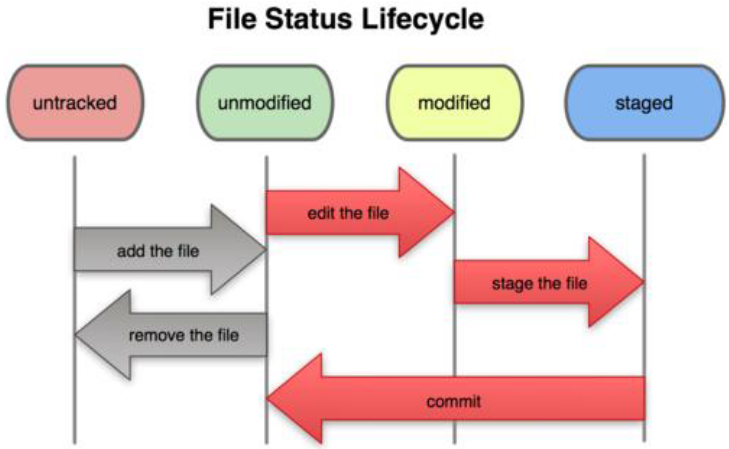
\includegraphics[width=0.8\textwidth]{gitf.png}
% %\vspace{-0.5cm}
% %\caption{\tiny Fuente: https://en.wikipedia.org/wiki}
% %\end{figure}
% \end{center}
%%\end{columns}
%\end{frame}	
%
%%---
%\section{\gih}
%\begin{frame}[c]{\gih}
%\begin{columns}
%\column{0.8\textwidth}
%\begin{block}{\gih}
%\begin{itemize}
%    \item \href{http://www.github.com}{\gih} es una p\'agina web de libre acceso para archivar repositorios online.
%    \item Muchos repositorios de codigo abierto como el kernel de Linux usan \gih.
%    \item ?`Es necesario tener \gih\ para usar \gi? \textbf{No!}
%    \begin{itemize}
%        \item Se puede usar \gi\ localmente, o  
%        \item se puede configurar un servidor para compartir archivos.
%    \end{itemize}     
%\end{itemize}
%\end{block}
%\column{0.2\textwidth}
%\begin{center}
% 
\includegraphics[width=0.8\textwidth]{ghub.png}
% \end{center}
%\end{columns}
%\end{frame}
%
%
%%---
%\section{Commandos b\'asicos en \gi}
%\begin{frame}[c]{Workflow b\'asico en \gi}
%\begin{block}{Workflow b\'asico en \gi}
%\begin{enumerate}
%    \item \alert{Pull} el directorio \gi\ del servidor remoto (opcional).
%    \item \alert{Modificar} los archivos en el directorio de trabajo
%    \item \alert{Stage} archivos. Adicionar un copia del archivo a la staging area.
%    \item Hacer un \alert{commit}, el cual toma los archivos en la staging area y archiva la copia en el directorio de \gi. 
%    \item \alert{Push} el directorio \gi\ a el servidor remoto (opcional).
%\end{enumerate}
%\end{block}
%\begin{center}
% 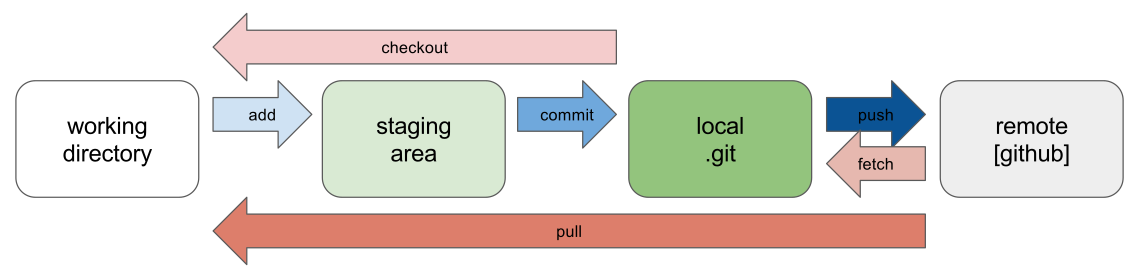
\includegraphics[width=\textwidth]{workflow.png}
%\end{center}
%\end{frame}	
%
%\begin{frame}[c]{Configuraci\'on inicial en \gi}
%\begin{block}{Alistarse para usar \gi}
%    \begin{enumerate}
%    \item Introducir \texttt{username} y \texttt{email} para ser usado por \gi\ cuando se haga un \texttt{commit}.\\
%     \co{\$ git config --global user.name “Luis Morales”}\\ %\vspace{0.3cm}
%     \co{\$ git config --global user.email lmoralesm@unal.edu.co}
%     \begin{itemize}
%         \item Para verificar la configuraci\'on:\\
%              \co{\$ git config -list}
%         \item Esta configuraci\'on es para todos los proyectos \gi.
%         \item La configuraci\'on anterior puede ser para un proyecto determinado si no se usa la opci\'on \co{-{}-global}
%         \item Adem\'as en la configuraci\'on inicial se puede escoger el editor para escribir mensajes en commit:
%         \co{\$ git config -{}-global core.editor vim}
%     \end{itemize}
%    \end{enumerate}
%\end{block}
%\end{frame}	
%
%\begin{frame}[c]{Crear una copia local del repositorio}
%\begin{block}{Crear copia local del repositorio \gi}
%\begin{enumerate}
%    \item Dos escenarios posibles:
%    \begin{enumerate}
%        \item Clonar un repositorio existente en su directorio local:\\
%        \co{\$ git clone <url> [local\_dir\_name]}\\
%        Crea el directorio \texttt{local\_dir\_name}, el cual contiene una copia de los archivos del repo original, y un directorio \texttt{.git}.
%        \item Crear un repositorio \gi\ en el directorio actual:\\
%        \co{\$ git init}\\
%        Crea el directorio \texttt{.git} en el directorio actual.  
%    \end{enumerate}
%\end{enumerate}
%\end{block}
%\end{frame}	
%
%\begin{frame}[c]{Commit archivos}
%\begin{block}{Commit archivos en el repo local}
%\begin{enumerate}
%    \item Una ves creado el directorio, se puede:
%    \begin{enumerate}
%        \item Se pueden crear archivos dentro del repositorio y adicionarlos a la staging \'area: \\
%        \co{\$ git add README.md file1.c}\\
%        Toma un snapshop de estos archivos en este instante de tiempo y los adiciona a la staging \'area.
%        \item Commit cambios en el repo (mover los staged cambios al repo)
%        \co{\$ git commit -m "initial project version"}\\
%    \end{enumerate}
%    Para unstage cambios (deshacer cambios) en un archivo antes de commit este):\\
%    \co{\$ git reset HEAD -{}- filename}
%    Para deshacer cambios en un archivo despu\'es de commit este:\\
%    \co{\$ git checkout -{}- filename}
%\end{enumerate}
%\end{block}
%\end{frame}	
%
%\begin{frame}[c]{Status y Diff}
%\begin{block}{Status y Diff}
%\begin{itemize}
%    \item Para mirar el \texttt{status} de los archivos en el directorio de trabajo o repo y la staging area:\\
%    \co{\$ git status} o \\
%    \co{\$ git status -s}\\
%    donde la opci\'on \co{-s} muestra una versi\'on del archivo en la staging \'area.
%    \item Para ver cual archivo ha sido modificado pero no est\'a en la staging \'area:\\
%    \co{\$ git diff}
%    \item Para ver cambios que ya estan en la staging \'area:\\
%    \co{\$ git diff}
%\end{itemize}
%\end{block}
%\end{frame}	
%
%\begin{frame}[c]{Chequeando los \texttt{logs}}
%\begin{block}{Chequeando los \texttt{logs}}
%\texttt{log} es un comando en \gi\ que permite conocer los cambios hechos en el repo. Algunos comandos importantes:
%\begin{itemize}
%    \item Chequeando la versi\'on larga de \texttt{logs}:\\
%    \co{\$ git log}
%    \item Chequeando la versi\'on larga de \texttt{logs}:\\
%    \co{\$ git log -{}-oneline}
%    %\begin{center}
%    %\includegraphics[width=\textwidth]{}
%    %\end{center}
%    \item Para mostrar los 5 m\'as recientes cambios:\\
%    \co{\$ git log -5}
%\end{itemize}
%Notas:
%\begin{enumerate}
%    \item Los cambios son listado de acuerdo con el commitID \#.
%    \item Todos los cambios hechos en el repo antes de haber sido clonado o jalado estan incluidos en \texttt{logs}.  
%\end{enumerate}
%\end{block}
%\end{frame}	
%
%\begin{frame}[c]{Pulling y pushing}
%\begin{block}{Pulling y pushing}
%\texttt{pull} y \texttt{push} son dos comandos que permiten jalar el repo de un servidor externo y enviar cambios a el repo, respectivamente. Buenas pr\'acticas en el uso de estos comandos son:
%\begin{enumerate}
%    \item \texttt{Add} y \texttt{commit} los cambios al repo local.
%    \item \texttt{pull} del repo remoto para obtener los cambios mas recientes. En caso de conflictos, \texttt{add} y \texttt{commit} estos al repo. 
%    \item \texttt{push} los cambios al repo remoto.
%\end{enumerate}
%Para incluir los cambios m\'as recientes del repo remoto en el repo local:\\
%\begin{enumerate}
%    \item Para bajar el contenido del repo remoto al repo local (optional):\\
%    \co{\$ git fetch}
%    \item Para bajar el contenido del repo remoto y actualizar el repo local:\\
%    \co{\$ git pull origin master}\\
%\end{enumerate}
%Para \texttt{push} los cambios realizados en el repo local a el repo remoto:\\
%\co{\$ git push origin master}
%\end{block}
%\end{frame}	
%
%\begin{frame}[c]{Branching}
%\vspace{-0.3cm}
%\begin{block}{Branching}
%\texttt{branch} es un comando que permite crear ramificaciones dentro del repo local para hacer cambios experimentales en el.
%\begin{itemize}
%    \item Para crear un \texttt{branch} llamado e.g. experiment1:\\
%    \co{\$ git branch experiment1}
%    \item Para listar todos los branches en el repo:\\
%    \co{\$ git branch}\\
%    Note que * indica el branch actual
%    \item Para cambiar al branch \texttt{experiment1}:\\
%    \co{\$ git checkout experiment1}
%    \item Para introducir los cambios hechos en  \texttt{experiment1} dentro del branch \texttt{master}:\\
%    \co{\$ git checkout master}\\
%    \co{\$ git merge experiment1}      
%\end{itemize}
%Notas:
%\begin{enumerate}
%    \item \co{\$ git log -{}-graph} puede ser usado para mostrar los branches gr\'aficamente. 
%    \item Los branches est\'an solo en el repo local.
%\end{enumerate}
%\end{block}
%\end{frame}	
%
%\begin{frame}[c]{Resumen}
%\vspace{-0.2cm}
%\begin{block}{Resumen}
%Configuraci\'on inicial y clonaci\'on
%\begin{enumerate}
%    \item \co{\$ git config -{}-global user.name “Your Name”}
%    \item \co{\$ git config --global user.email youremail@unal.edu.co}
%    \item \co{\$ git clone https://github.com/hydsrg/hyds-repo.git}
%\end{enumerate}
%Editar y visualizar cambios \texttt{hyds-repo}
%\begin{enumerate}
%    \item \co{\$ git log}; \co{\$ git log -{}-oneline}
%    \item Create a file, e.g. \texttt{filename.txt}
%    \item \co{\$ git status}; \co{\$ git status –s}
%    \item Agregar el archivo al repo (staging area): \co{git add filename.txt}
%    \item \co{\$ git status}; \co{\$ git status –s}
%    \item \texttt{commit} el archivo al repo local:\\
%    \co{\$ git commit –m “added filename.txt file”}
%    \item \co{\$ git status}; \co{\$ git status –s}; \co{\$ git log -{}-oneline}
%\end{enumerate}
%\end{block}
%\end{frame}	
%
%\begin{frame}[c]{Resumen}
%\begin{block}{Resumen}
%Pulling y pushing los cambios
%\begin{enumerate}
%    \item \texttt{pull} de un repo remoto: \co{\$ git pull origin master}
%    \item \texttt{push} hacia un repo remoto: \co{\$ git push origin master}
%\end{enumerate}
%\end{block}
%\end{frame}	

%
\end{document}


